\documentclass[french, 12pt]{article}

\usepackage{fontspec}
\usepackage{arsenal}
\usepackage{tikz}
\usepackage{babel}
% minimum width=3cm
\usetikzlibrary{positioning,shapes}
%
\tikzstyle{startstop} = [rectangle, rounded corners, minimum width=4cm, minimum height=1cm,text centered, draw=black, fill=green!30]
\tikzstyle{decision} = [diamond, minimum width=4cm, minimum height=1cm, text centered, draw=black, fill=green!30]
\tikzstyle{process} = [rectangle, minimum width=4cm, minimum height=1cm, text centered, draw=black, fill=orange!30]
\tikzstyle{arrow} = [thick,->,>=stealth]


\begin{document}
%
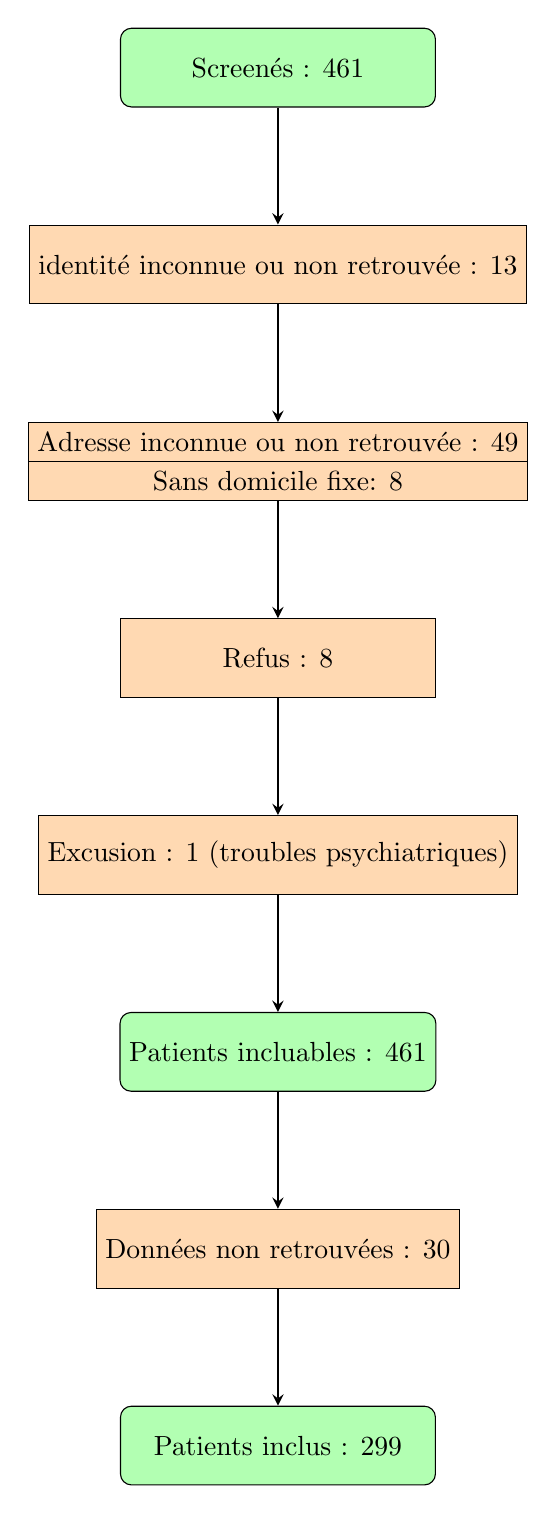
\begin{tikzpicture}
\node (screen) at (4,0) [draw, startstop,
minimum height=1 cm] {Screenés : 461};
%
\node (ident) at (4,-2.5) [draw, process,
minimum height=1 cm] {identité inconnue ou non retrouvée : 13};

\node (adresse) at (4,-5) [rectangle split,rectangle split parts=2, minimum width=4cm, minimum height=1cm, text centered, draw=black, fill=orange!30] {Adresse inconnue ou non retrouvée : 49 \nodepart{second}
Sans domicile fixe: 8};



\node (refus) at (4, -7.5) [draw, process,
minimum height=1 cm] {Refus : 8};
%
\node (psy) at (4,-10) [draw, process,
minimum height=1 cm] {Excusion : 1 (troubles psychiatriques)};
%
\node (inclus1) at (4,-12.5) [draw, startstop,
minimum height=1 cm] {Patients incluables : 461};
%
\node (erreur) at (4,-15) [draw, process,
minimum height=1 cm] {Données non retrouvées : 30};
%
\node (inclusf) at (4,-17.5) [draw, startstop,
minimum height=1 cm] {Patients inclus : 299};
%
\draw [arrow] (screen) -- (ident);
\draw [arrow] (ident) -- (adresse);
\draw [arrow] (adresse) -- (refus);
\draw [arrow] (refus) -- (psy);
\draw [arrow] (psy) -- (inclus1);
\draw [arrow] (inclus1) -- (erreur);
\draw [arrow] (erreur) -- (inclusf);

\end{tikzpicture}
%
\end{document}
